\documentclass[11pt,a4paper]{article}
\usepackage[utf8]{inputenc}
\usepackage[greek,english]{babel}
\usepackage{alphabeta}
\usepackage{graphicx}
\usepackage{listings}
\usepackage{xcolor}
\usepackage{hyperref}
\usepackage{geometry}
\geometry{a4paper, margin=0.8in}

\definecolor{backcolour}{rgb}{0.97,0.97,0.95}
\definecolor{codegreen}{rgb}{0,0.6,0}
\definecolor{codegray}{rgb}{0.5,0.5,0.5}

\lstdefinestyle{mystyle}{
    backgroundcolor=\color{backcolour},
    basicstyle=\ttfamily\scriptsize,
    breaklines=true,
    numbers=left,
    numberstyle=\tiny\color{codegray},
    numbersep=5pt,
    showstringspaces=false,
    tabsize=2
}
\lstset{style=mystyle}

\hypersetup{
    colorlinks=true,
    linkcolor=blue,
    urlcolor=cyan,
}

\begin{document}
\selectlanguage{greek}

% =========================================================
% ΕΞΩΦΥΛΛΟ
% =========================================================
\begin{titlepage}
    \centering
    \vspace*{1.5cm}
    {\large ΠΑΝΕΠΙΣΤΗΜΙΟ ΠΑΤΡΩΝ}\\[0.2cm]
    {\large ΤΜΗΜΑ ΜΗΧΑΝΙΚΩΝ Η/Υ ΚΑΙ ΠΛΗΡΟΦΟΡΙΚΗΣ}\\[1.5cm]
    {\large Μάθημα: Συστήματα Διαχείρισης Μεγάλων Δεδομένων}\\[2cm]
    {\Large \bfseries ΤΕΛΙΚΗ ΑΝΑΦΟΡΑ \textlatin{PROJECT}}\\[0.5cm]
    {\Large \bfseries Επεξεργασία Δεδομένων Ροής με \textlatin{Kafka}, \textlatin{Spark} και \textlatin{MongoDB}}\\[2.5cm]
    \begin{minipage}{0.45\textwidth}
        \begin{flushleft}\large
            \emph{Φοιτητής:}\\
            Κωνσταντίνος Κολύβρας 1103826
        \end{flushleft}
    \end{minipage}
    \hfill
    \begin{minipage}{0.45\textwidth}
        \begin{flushright}\large
            \emph{Υπεύθυνοι Καθηγητές:}\\
            Β. Μεγαλοοικονόμου\\
            Ε. Ζαχαράκη
        \end{flushright}
    \end{minipage}
    \vfill
    {\large Ιούνιος 2026}
\end{titlepage}

% =========================================================
% 1. ΑΡΧΙΤΕΚΤΟΝΙΚΗ
% =========================================================
\section{Περιγραφή Αρχιτεκτονικής}

Η εφαρμογή υλοποιεί μια \textlatin{real-time stream processing pipeline} με τέσσερα επίπεδα:

\begin{itemize}
    \item \textbf{\textlatin{Data Producer} (\textlatin{producer.py})}: Ο \textlatin{UXSIM traffic simulator} παράγει δεδομένα κίνησης οχημάτων. Τα αποτελέσματα φιλτράρονται (μόνο οχήματα με $v > 0$) και αποστέλλονται ως \textlatin{JSON records} στο \textlatin{Redpanda topic} \texttt{\textlatin{vehicle\_positions}} μέσω της βιβλιοθήκης \textlatin{kafka-python}.

    \item \textbf{\textlatin{Message Broker} (\textlatin{Redpanda})}: Το \textlatin{Redpanda} είναι ένας \textlatin{broker} συμβατός με το \textlatin{Kafka API}, ο οποίος λαμβάνει και αποθηκεύει προσωρινά τα μηνύματα. Εκτελείται μέσω \textlatin{Docker} και εκθέτει δύο \textlatin{listeners}: εσωτερικά στο \texttt{\textlatin{redpanda:9092}} (για το \textlatin{Spark}) και εξωτερικά στο \texttt{\textlatin{localhost:19092}} (για τον \textlatin{producer}).

    \item \textbf{\textlatin{Stream Processing} (\textlatin{spark\_streaming.py})}: Το \textlatin{Apache Spark Structured Streaming} καταναλώνει τα δεδομένα από το \textlatin{topic}, ορίζει \textlatin{schema} για το \textlatin{parsing} των \textlatin{JSON} μηνυμάτων και υπολογίζει στατιστικά (\textlatin{vcount}, \textlatin{vspeed}) ανά \textlatin{time} και \textlatin{link} με \texttt{\textlatin{groupBy}}.

    \item \textbf{\textlatin{NoSQL Database} (\textlatin{MongoDB})}: Αποθηκεύει τα \textlatin{raw data} στο \textlatin{collection} \texttt{\textlatin{raw\_data}} και τα επεξεργασμένα \textlatin{stats} στο \textlatin{collection} \texttt{\textlatin{stats}}, και τα δύο στη βάση \texttt{\textlatin{traffic}}.
\end{itemize}

% =========================================================
% 2. ΣΧΕΔΙΑΣΤΙΚΕΣ ΕΠΙΛΟΓΕΣ
% =========================================================
\section{Σχεδιαστικές Επιλογές}

\begin{itemize}
    \item \textbf{Δίκτυο \textlatin{UXSIM}}: Δημιουργήθηκε δίκτυο 4×4 \textlatin{grid} με 4 \textlatin{intersections} (\texttt{\textlatin{I1}}-\texttt{\textlatin{I4}}) και \textlatin{traffic signals} με κύκλο 60 δευτερολέπτων. Η τυχαία ζήτηση ορίζεται κάθε 30 δευτερόλεπτα. Η εξαγωγή γίνεται με τη \texttt{\textlatin{vehicles\_to\_pandas()}} και επιστρέφει τα πεδία: \texttt{\textlatin{t}}, \texttt{\textlatin{veh}}, \texttt{\textlatin{link}}, \texttt{\textlatin{x}}, \texttt{\textlatin{v}}.

    \item \textbf{\textlatin{Spark Schema}}: Ορίστηκε \textlatin{StructType} \textlatin{schema} για το \textlatin{parsing} των \textlatin{JSON} μηνυμάτων, εξασφαλίζοντας σωστούς τύπους (\textlatin{DoubleType} για \texttt{\textlatin{t}}, \texttt{\textlatin{x}}, \texttt{\textlatin{s}}, \texttt{\textlatin{v}} και \textlatin{StringType} για \texttt{\textlatin{link}}, \texttt{\textlatin{orig}}, \texttt{\textlatin{dest}}).

    \item \textbf{\textlatin{MongoDB Sinks}}: Τα \textlatin{raw data} γράφονται με \texttt{\textlatin{outputMode("append")}}. Τα \textlatin{stats} γράφονται μέσω \texttt{\textlatin{foreachBatch}}, καθώς το \textlatin{update mode} με \textlatin{aggregations} δεν υποστηρίζεται απευθείας από τον \textlatin{MongoDB Spark connector}.
\end{itemize}

% =========================================================
% 3. ΠΡΟΒΛΗΜΑΤΑ ΚΑΙ ΛΥΣΕΙΣ
% =========================================================
\section{Προβλήματα που Αντιμετωπίστηκαν και Λύσεις}

\begin{enumerate}
    \item \textbf{\textlatin{Numpy JSON Serialization}}: Οι τύποι \texttt{\textlatin{np.int64}} και \texttt{\textlatin{np.float64}} του \textlatin{UXSIM} δεν γίνονται \textlatin{serialize} από την τυπική βιβλιοθήκη \textlatin{json} της \textlatin{Python}. Υλοποιήθηκε η συνάρτηση \texttt{\textlatin{convert(obj)}} που μετατρέπει τις τιμές σε \textlatin{native int/float} πριν την αποστολή.

    \item \textbf{Φιλτράρισμα Κινούμενων Οχημάτων}: Η εκφώνηση ζητά αποστολή μόνο οχημάτων σε κίνηση. Προστέθηκε έλεγχος \textlatin{v > 0} στον \textlatin{producer} πριν το \texttt{\textlatin{send()}}, ώστε να αποκλείονται τα σταματημένα οχήματα.

    \item \textbf{\textlatin{Docker Networking}}: Ο \textlatin{Spark consumer} τρέχει σε \textlatin{Docker container} ενώ ο \textlatin{producer} τρέχει στο \textlatin{host OS}. Ρυθμίστηκαν διπλοί \textlatin{advertised listeners} στο \textlatin{Redpanda} (\texttt{\textlatin{redpanda:9092}} εσωτερικά, \texttt{\textlatin{localhost:19092}} εξωτερικά).
\end{enumerate}

\newpage

% =========================================================
% 4. SCREENSHOTS
% =========================================================
\section{\textlatin{Screenshots} και Αποτελέσματα}

\subsection{\textlatin{Redpanda}: Λήψη Μηνυμάτων στο \textlatin{Topic}}

\begin{figure}[htbp]
    \centering
    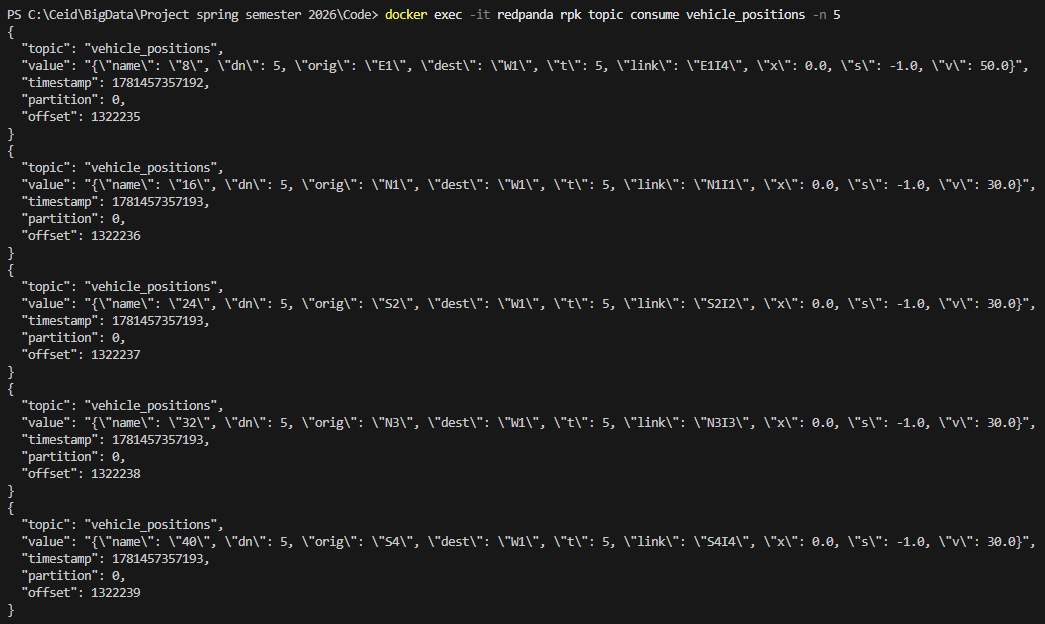
\includegraphics[width=0.85\textwidth,height=7.5cm,keepaspectratio]{RedPandaTopic.png}
    \caption{Λήψη \textlatin{JSON} μηνυμάτων στο \textlatin{Redpanda topic} \texttt{\textlatin{vehicle\_positions}} μέσω \textlatin{rpk topic consume}.}
\end{figure}

\subsection{\textlatin{Spark}: Αποτελέσματα \textlatin{Streaming Console}}

\begin{figure}[htbp]
    \centering
    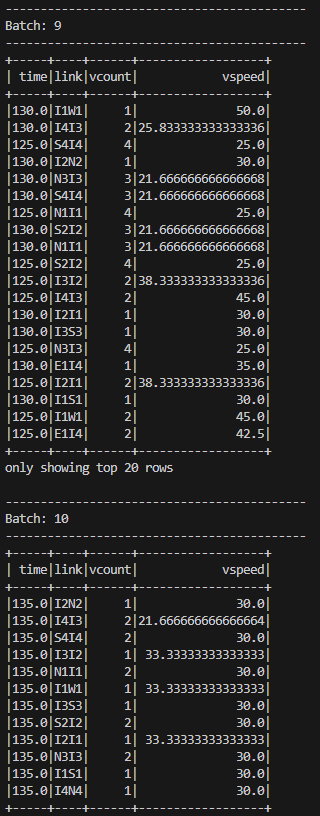
\includegraphics[width=0.85\textwidth,height=7.5cm,keepaspectratio]{SparkStreamingLogs.png}
    \caption{\textlatin{Micro-batches} από τον \textlatin{Spark Structured Streaming consumer}, με στατιστικά (\textlatin{time}, \textlatin{link}, \textlatin{vcount}, \textlatin{vspeed}) ανά ακμή.}
\end{figure}

\newpage

\subsection{\textlatin{MongoDB}: \textlatin{Collections} και \textlatin{Documents}}

\begin{figure}[htbp]
    \centering
    
\includegraphics[width=0.75\textwidth,height=6cm,keepaspectratio]{MongoDBstatscollection.png}
    \caption{Τα \textlatin{collections} \texttt{\textlatin{raw\_data}} και \texttt{\textlatin{stats}} στη βάση \texttt{\textlatin{traffic}} της \textlatin{MongoDB}.}
\end{figure}

\begin{figure}[htbp]
    \centering
    \begin{minipage}{0.48\textwidth}
        \centering
        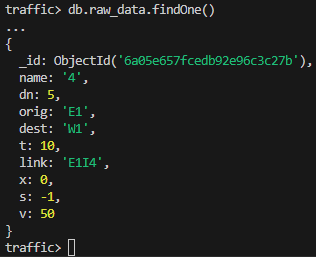
\includegraphics[width=\linewidth,height=5.5cm,keepaspectratio]{RawData1.png}
        \caption{\textlatin{Document} από το \textlatin{collection} \texttt{\textlatin{raw\_data}}.}
    \end{minipage}\hfill
    \begin{minipage}{0.48\textwidth}
        \centering
        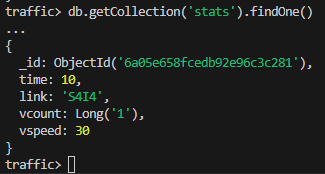
\includegraphics[width=\linewidth,height=5.5cm,keepaspectratio]{RawData2.png}
        \caption{\textlatin{Document} από το \textlatin{collection} \texttt{\textlatin{stats}}.}
    \end{minipage}
\end{figure}


% =========================================================
% 5. AGGREGATION QUERIES
% =========================================================
\section{\textlatin{Aggregation Queries} στη \textlatin{MongoDB}}

\noindent
\begin{minipage}[t]{0.48\textwidth}
\subsection{\textlatin{Query} 1: Μέση Ταχύτητα ανά \textlatin{Link}}
\begin{otherlanguage}{english}
\begin{lstlisting}
db.getCollection('stats').aggregate([
  { $group: { _id: "$link",
              avg_speed: { $avg: "$vspeed" },
              total_records: { $sum: "$vcount" } } },
  { $sort: { avg_speed: -1 } }
])
\end{lstlisting}
\end{otherlanguage}
\begin{center}
    
\includegraphics[width=\linewidth,height=5.5cm,keepaspectratio]{AggregationQuery1.png}\\[2pt]
    {\small Αποτελέσματα \textlatin{Query} 1.}
\end{center}
\end{minipage}
\hfill
\begin{minipage}[t]{0.48\textwidth}
\subsection{\textlatin{Query} 2: Οι 5 Πιο Συμφορημένες Ακμές}
\begin{otherlanguage}{english}
\begin{lstlisting}
db.getCollection('stats').aggregate([
  { $group: { _id: "$link",
              avg_density: { $avg: "$vcount" },
              max_vehicles: { $max: "$vcount" } } },
  { $sort: { avg_density: -1 } },
  { $limit: 5 }
])
\end{lstlisting}
\end{otherlanguage}
\begin{center}
    
\includegraphics[width=\linewidth,height=5.5cm,keepaspectratio]{AggregationQuery2.png}\\[2pt]
    {\small Αποτελέσματα \textlatin{Query} 2.}
\end{center}
\end{minipage}

% =========================================================
% 6. BONUS: REST API
% =========================================================
\section{Προαιρετικό (\textlatin{Bonus}): \textlatin{REST API} με \textlatin{FastAPI}}

Υλοποιήθηκε απλό \textlatin{REST API} (αρχείο \texttt{\textlatin{api.py}}) με τη βιβλιοθήκη \textlatin{FastAPI}, το οποίο διαβάζει δεδομένα απευθείας από τη \textlatin{MongoDB} και εκθέτει τα παρακάτω \textlatin{endpoints}:

\begin{itemize}
    \item \texttt{\textlatin{GET /stats}} — Επιστρέφει τα τελευταία \textlatin{aggregated stats} (\textlatin{time}, \textlatin{link}, \textlatin{vcount}, \textlatin{vspeed}).
    \item \texttt{\textlatin{GET /stats/top5}} — Επιστρέφει τις 5 πιο συμφορημένες ακμές (κατά μέσο αριθμό οχημάτων), μέσω \textlatin{MongoDB aggregation pipeline}.
    \item \texttt{\textlatin{GET /stats/avg-speed}} — Επιστρέφει τη μέση ταχύτητα ανά ακμή σε όλο το διάστημα εξομοίωσης.
    \item \texttt{\textlatin{GET /raw}} — Επιστρέφει τα τελευταία \textlatin{raw} αρχεία θέσης οχημάτων.
\end{itemize}

Το \textlatin{API} εκτελείται ως ξεχωριστό \textlatin{service} στο \textlatin{Docker Compose} (\texttt{\textlatin{traffic-api}}, \textlatin{port} \textlatin{8000}) και συνδέεται στη \textlatin{MongoDB} μέσω της μεταβλητής περιβάλλοντος \texttt{\textlatin{MONGO\_URI}}. Προσβάσιμο στο \texttt{\textlatin{http://localhost:8000/docs}} (αυτόματο \textlatin{Swagger UI}).

% =========================================================
% 7. ΣΥΜΠΕΡΑΣΜΑ
% =========================================================
\section{Συμπέρασμα}

Η \textlatin{pipeline} λειτούργησε επιτυχώς από άκρο σε άκρο. Ο \textlatin{UXSIM simulator} παρήγαγε ρεαλιστικά δεδομένα κυκλοφορίας, τα οποία ο \textlatin{Spark Structured Streaming consumer} κατανάλωσε σε \textlatin{real-time}, υπολόγισε στατιστικά ανά ακμή και τα αποθήκευσε στη \textlatin{MongoDB}. Τα \textlatin{aggregation queries} αναδεικνύουν τις πιο συμφορημένες ακμές του δικτύου. Επιπλέον, υλοποιήθηκε \textlatin{REST API} (\textlatin{bonus}) που εκθέτει τα δεδομένα της \textlatin{MongoDB} μέσω \textlatin{HTTP endpoints}.

\end{document}
